\documentclass{article}
\usepackage[a3paper,landscape,margin=8mm]{geometry}
\usepackage{tikz}
\usetikzlibrary{arrows.meta,backgrounds,fit,positioning}
\pagestyle{empty}

\definecolor{clientbg}{RGB}{232,242,255}
\definecolor{appbg}{RGB}{235,247,238}
\definecolor{msgbg}{RGB}{255,246,224}
\definecolor{databg}{RGB}{242,236,255}
\definecolor{bootbg}{RGB}{244,244,244}
\definecolor{extbg}{RGB}{255,235,232}
\definecolor{linegray}{RGB}{80,88,99}

\tikzset{
  group/.style={
    rounded corners=3pt,
    draw=linegray,
    line width=0.7pt,
    inner sep=6pt
  },
  box/.style={
    rounded corners=2pt,
    draw=linegray,
    fill=white,
    line width=0.6pt,
    align=center,
    minimum width=3.4cm,
    minimum height=1.1cm,
    text width=3.2cm,
    font=\sffamily\scriptsize
  },
  widebox/.style={
    box,
    minimum width=4.4cm,
    text width=4.2cm
  },
  smallbox/.style={
    box,
    minimum width=2.9cm,
    text width=2.7cm,
    minimum height=0.9cm
  },
  title/.style={
    font=\sffamily\bfseries\Large,
    align=left
  },
  grouptitle/.style={
    font=\sffamily\bfseries\small,
    align=left
  },
  flow/.style={
    -{Stealth[length=2.8mm]},
    draw=linegray,
    line width=0.75pt
  },
  async/.style={
    flow,
    dashed
  },
  dataflow/.style={
    flow,
    draw=purple!70!black
  },
  extflow/.style={
    flow,
    draw=red!65!black
  },
  label/.style={
    fill=white,
    inner sep=1.4pt,
    font=\sffamily\tiny,
    align=center,
    text=linegray
  }
}

\begin{document}
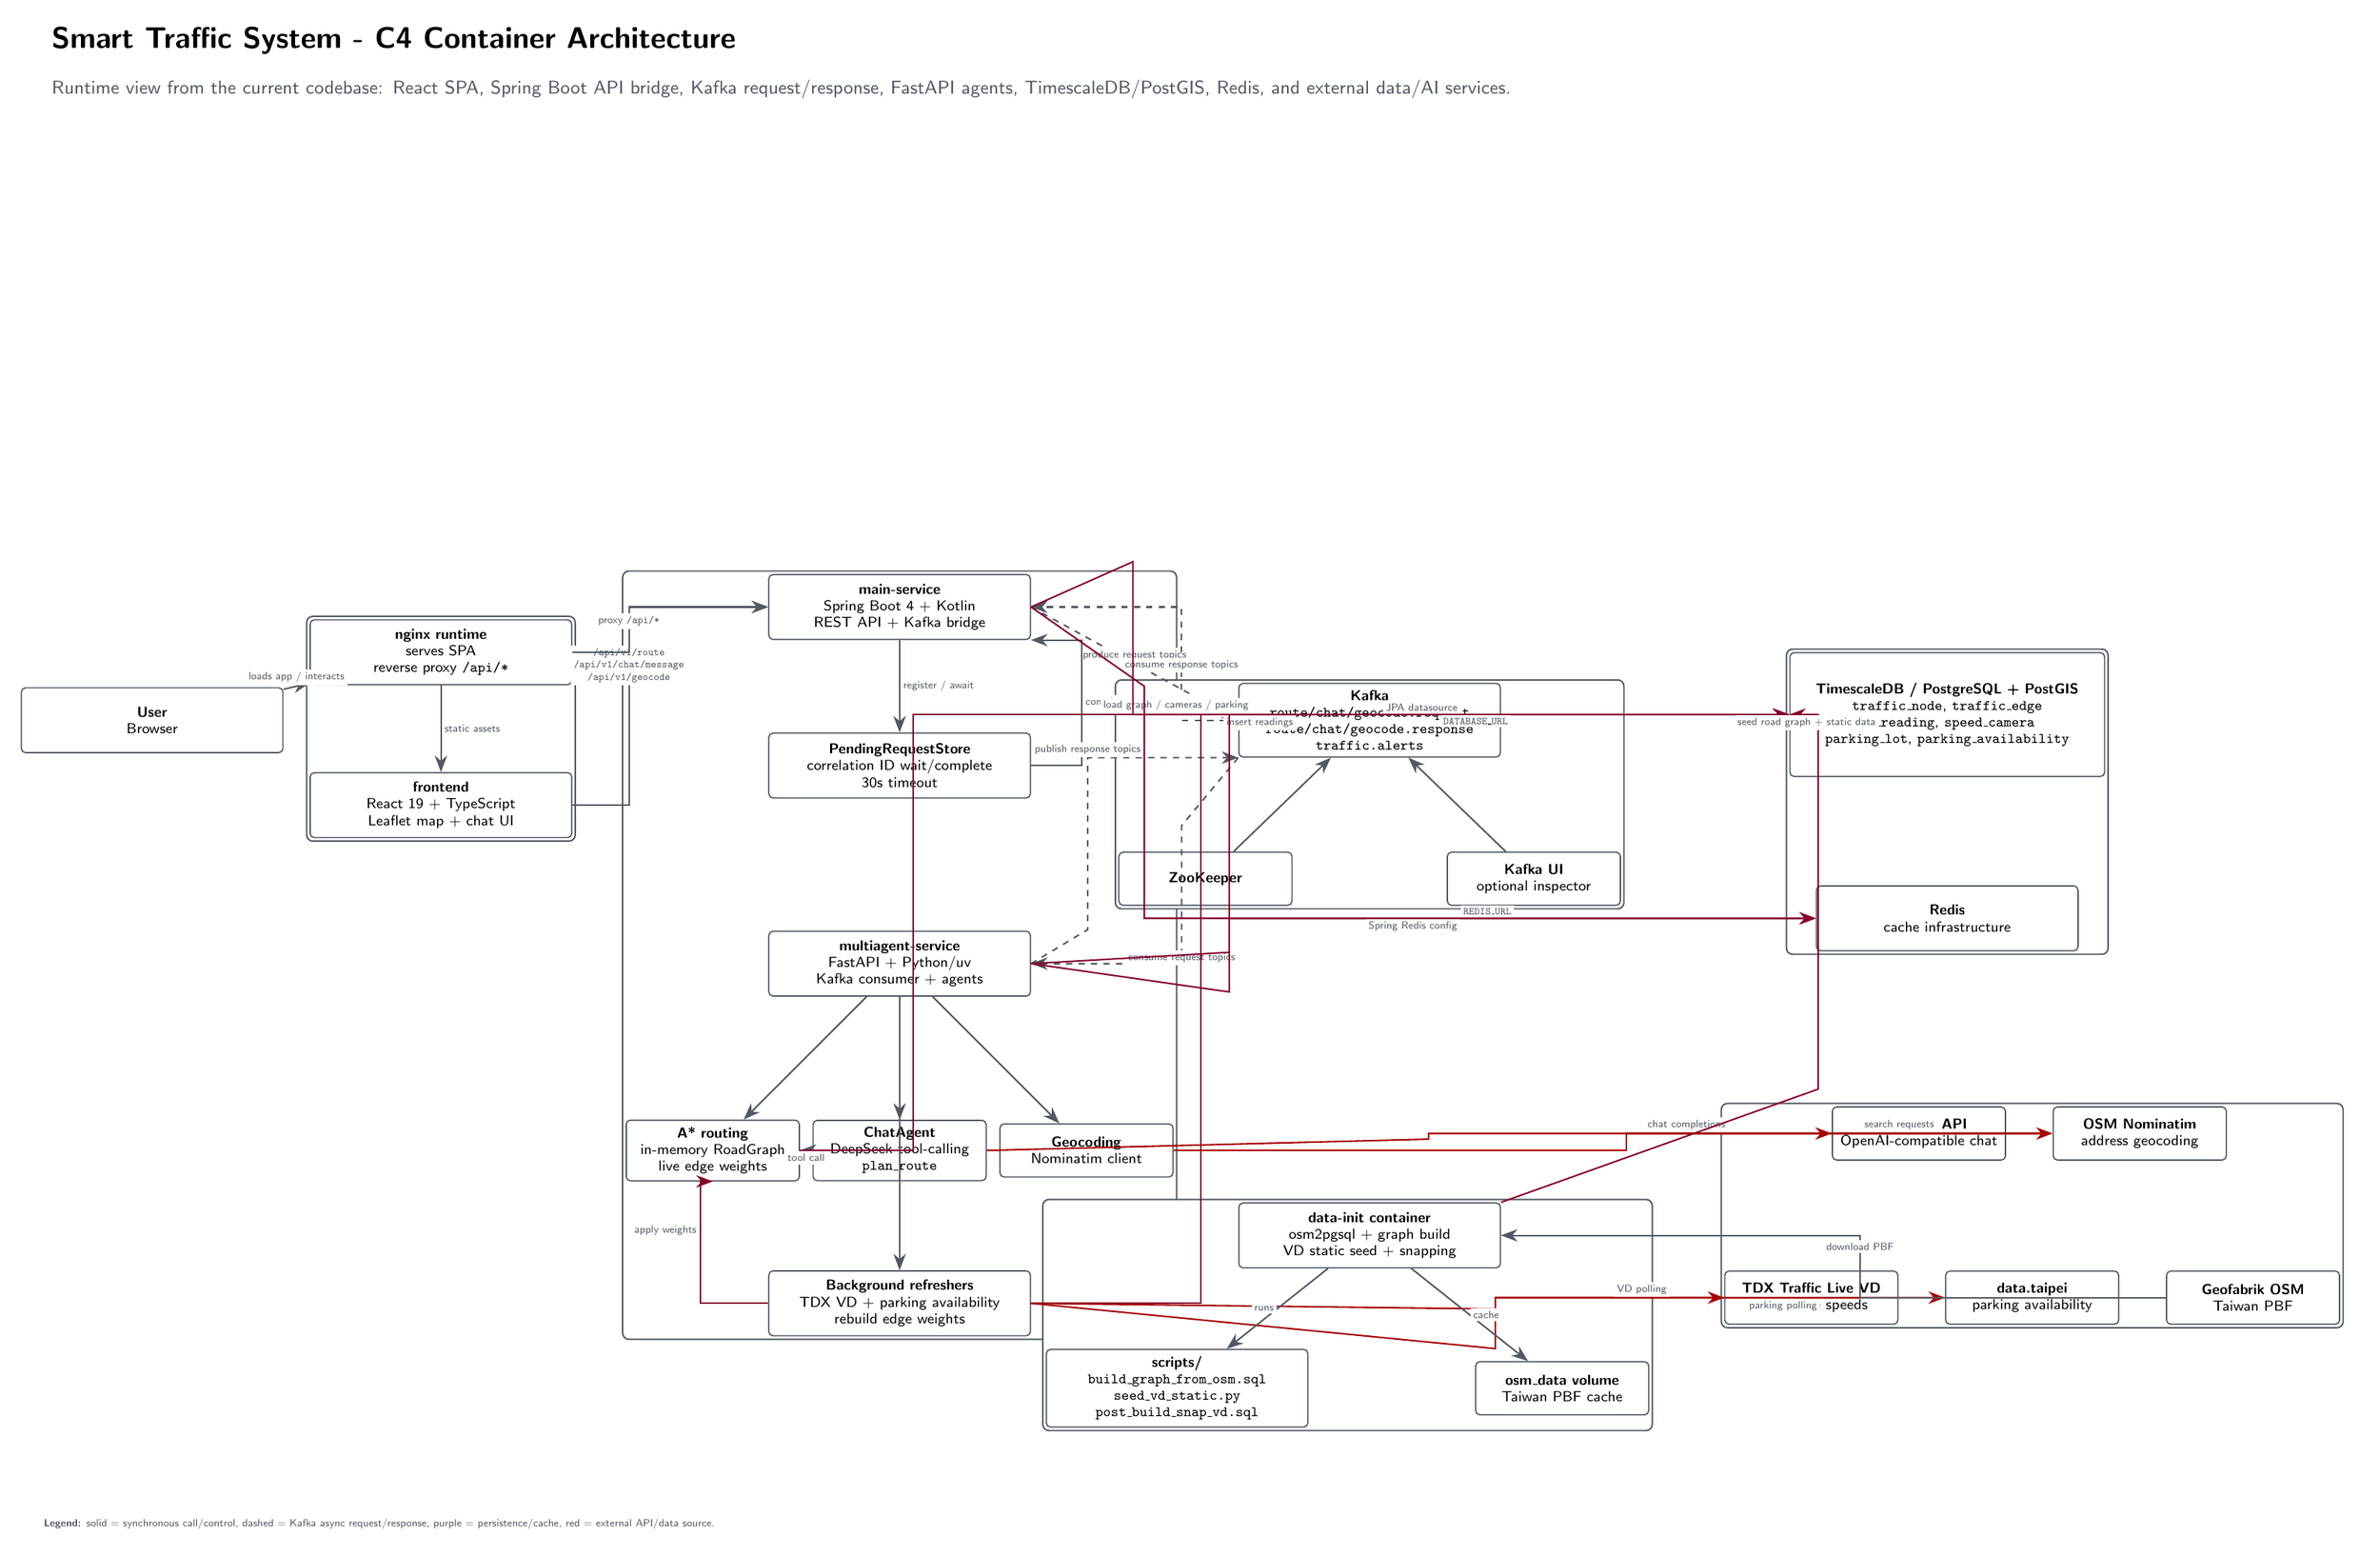
\begin{tikzpicture}[x=0.96cm,y=0.96cm]
  \node[title,anchor=west] at (0,27.2) {Smart Traffic System - C4 Container Architecture};
  \node[font=\sffamily\small,align=left,text=linegray,anchor=west,text width=39cm] at (0,26.35)
    {Runtime view from the current codebase: React SPA, Spring Boot API bridge, Kafka request/response, FastAPI agents, TimescaleDB/PostGIS, Redis, and external data/AI services.};

  % User
  \node[widebox,fill=white] (user) at (1.9,15.2) {\textbf{User}\\Browser};

  % Client group
  \node[widebox] (nginx) at (7.0,16.4) {\textbf{nginx runtime}\\serves SPA\\reverse proxy \texttt{/api/*}};
  \node[widebox] (spa) at (7.0,13.7) {\textbf{frontend}\\React 19 + TypeScript\\Leaflet map + chat UI};
  \begin{scope}[on background layer]
    \node[group,fill=clientbg,fit=(nginx)(spa),label={[grouptitle]north west:Client}] {};
  \end{scope}

  % Application group
  \node[widebox] (main) at (15.1,17.2) {\textbf{main-service}\\Spring Boot 4 + Kotlin\\REST API + Kafka bridge};
  \node[widebox] (pending) at (15.1,14.4) {\textbf{PendingRequestStore}\\correlation ID wait/complete\\30s timeout};
  \node[widebox] (multi) at (15.1,10.9) {\textbf{multiagent-service}\\FastAPI + Python/uv\\Kafka consumer + agents};
  \node[smallbox] (routing) at (11.8,7.6) {\textbf{A* routing}\\in-memory RoadGraph\\live edge weights};
  \node[smallbox] (chat) at (15.1,7.6) {\textbf{ChatAgent}\\DeepSeek tool-calling\\\texttt{plan\_route}};
  \node[smallbox] (geocode) at (18.4,7.6) {\textbf{Geocoding}\\Nominatim client};
  \node[widebox] (refresh) at (15.1,4.9) {\textbf{Background refreshers}\\TDX VD + parking availability\\rebuild edge weights};
  \begin{scope}[on background layer]
    \node[group,fill=appbg,fit=(main)(pending)(multi)(routing)(chat)(geocode)(refresh),label={[grouptitle]north west:Application Services}] {};
  \end{scope}

  % Messaging group
  \node[widebox] (kafka) at (23.4,15.2) {\textbf{Kafka}\\\texttt{route/chat/geocode.request}\\\texttt{route/chat/geocode.response}\\\texttt{traffic.alerts}};
  \node[smallbox] (zk) at (20.5,12.4) {\textbf{ZooKeeper}};
  \node[smallbox] (kafkaui) at (26.3,12.4) {\textbf{Kafka UI}\\optional inspector};
  \begin{scope}[on background layer]
    \node[group,fill=msgbg,fit=(kafka)(zk)(kafkaui),label={[grouptitle]north west:Messaging}] {};
  \end{scope}

  % Data group
  \node[widebox,minimum width=5.3cm,text width=5.1cm,minimum height=2.1cm] (db) at (33.6,15.3)
    {\textbf{TimescaleDB / PostgreSQL + PostGIS}\\\texttt{traffic\_node}, \texttt{traffic\_edge}\\\texttt{vd\_reading}, \texttt{speed\_camera}\\\texttt{parking\_lot}, \texttt{parking\_availability}};
  \node[widebox] (redis) at (33.6,11.7) {\textbf{Redis}\\cache infrastructure};
  \begin{scope}[on background layer]
    \node[group,fill=databg,fit=(db)(redis),label={[grouptitle]north west:Data Stores}] {};
  \end{scope}

  % Bootstrap group
  \node[widebox] (datainit) at (23.4,6.1) {\textbf{data-init container}\\osm2pgsql + graph build\\VD static seed + snapping};
  \node[widebox] (scripts) at (20.0,3.4) {\textbf{scripts/}\\\texttt{build\_graph\_from\_osm.sql}\\\texttt{seed\_vd\_static.py}\\\texttt{post\_build\_snap\_vd.sql}};
  \node[smallbox] (osmcache) at (26.8,3.4) {\textbf{osm\_data volume}\\Taiwan PBF cache};
  \begin{scope}[on background layer]
    \node[group,fill=bootbg,fit=(datainit)(scripts)(osmcache),label={[grouptitle]north west:Bootstrap / One-shot Jobs}] {};
  \end{scope}

  % External systems
  \node[smallbox] (deepseek) at (33.1,7.9) {\textbf{DeepSeek API}\\OpenAI-compatible chat};
  \node[smallbox] (nominatim) at (37.0,7.9) {\textbf{OSM Nominatim}\\address geocoding};
  \node[smallbox] (tdx) at (31.2,5.0) {\textbf{TDX Traffic Live VD}\\Taipei live speeds};
  \node[smallbox] (taipei) at (35.1,5.0) {\textbf{data.taipei}\\parking availability};
  \node[smallbox] (geofabrik) at (39.0,5.0) {\textbf{Geofabrik OSM}\\Taiwan PBF};
  \begin{scope}[on background layer]
    \node[group,fill=extbg,fit=(deepseek)(nominatim)(tdx)(taipei)(geofabrik),label={[grouptitle]north west:External Systems}] {};
  \end{scope}

  % Main runtime flows
  \draw[flow] (user) -- node[label,above] {loads app / interacts} (nginx);
  \draw[flow] (nginx) -- node[label,right] {static assets} (spa);
  \draw[flow] (spa.east) -- ++(1.0,0) |- node[label,pos=0.3,above] {\texttt{/api/v1/route}\\\texttt{/api/v1/chat/message}\\\texttt{/api/v1/geocode}} (main.west);
  \draw[flow] (nginx.east) -- ++(1.0,0) |- node[label,pos=0.25,above] {proxy \texttt{/api/*}} (main.west);

  \draw[flow] (main) -- node[label,right] {register / await} (pending);
  \draw[async] (main.east) -- node[label,above] {produce request topics} (kafka.west);
  \draw[async] (kafka.west) -- ++(-1.0,0) |- node[label,pos=0.28,below] {consume response topics} (main.east);
  \draw[flow] (pending.east) -- ++(0.9,0) |- node[label,pos=0.25,right] {complete pending request} (main.south east);

  \draw[async] (kafka.south west) -- ++(-1.0,-1.2) |- node[label,pos=0.45,below] {consume request topics} (multi.east);
  \draw[async] (multi.east) -- ++(1.0,0.6) |- node[label,pos=0.5,above] {publish response topics} (kafka.south west);

  \draw[flow] (multi) -- (routing);
  \draw[flow] (multi) -- (chat);
  \draw[flow] (multi) -- (geocode);
  \draw[flow] (multi) -- (refresh);
  \draw[flow] (chat) -- node[label,below] {tool call} (routing);

  % Data flows
  \draw[dataflow] (routing.east) -- ++(2.0,0) |- node[label,pos=0.65,above] {load graph / cameras / parking} (db.west);
  \draw[dataflow] (refresh.east) -- ++(3.0,0) |- node[label,pos=0.55,below] {insert readings} (db.west);
  \draw[dataflow] (refresh.west) -- ++(-1.2,0) |- node[label,pos=0.3,left] {apply weights} (routing.south);
  \draw[dataflow] (main.east) -- ++(1.8,0.8) |- node[label,pos=0.72,above] {JPA datasource} (db.west);
  \draw[dataflow] (main.east) -- ++(2.0,-1.4) |- node[label,pos=0.7,below] {Spring Redis config} (redis.west);
  \draw[dataflow] (multi.east) -- ++(3.5,0.2) |- node[label,pos=0.72,below] {\texttt{DATABASE\_URL}} (db.west);
  \draw[dataflow] (multi.east) -- ++(3.5,-0.5) |- node[label,pos=0.72,above] {\texttt{REDIS\_URL}} (redis.west);

  % External flows
  \draw[extflow] (chat.east) -- ++(7.8,0.2) |- node[label,pos=0.82,above] {chat completions} (deepseek.west);
  \draw[extflow] (geocode.east) -- ++(8.0,0.0) |- node[label,pos=0.82,above] {search requests} (nominatim.west);
  \draw[extflow] (refresh.east) -- ++(8.2,-0.1) |- node[label,pos=0.82,above] {VD polling} (tdx.west);
  \draw[extflow] (refresh.east) -- ++(8.2,-0.8) |- node[label,pos=0.82,below] {parking polling} (taipei.west);

  % Bootstrap flows
  \draw[flow] (geofabrik.west) -- ++(-5.4,0) |- node[label,pos=0.35,above] {download PBF} (datainit.east);
  \draw[flow] (datainit) -- node[label,left] {runs} (scripts);
  \draw[dataflow] (datainit.north east) -- ++(5.6,2.0) |- node[label,pos=0.7,below] {seed road graph + static data} (db.west);
  \draw[flow] (datainit) -- node[label,right] {cache} (osmcache);

  % Infra relationships
  \draw[flow] (zk) -- (kafka);
  \draw[flow] (kafkaui) -- (kafka);

  % Legend
  \node[font=\sffamily\tiny,align=left,text=linegray,text width=15cm] at (7.8,1.0)
    {\textbf{Legend:} solid = synchronous call/control, dashed = Kafka async request/response, purple = persistence/cache, red = external API/data source.};
\end{tikzpicture}
\end{document}
